\documentclass[11pt]{article}

\usepackage[T1]{fontenc}
\usepackage[utf8]{inputenc}
\IfFileExists{lmodern.sty}{\usepackage{lmodern}}{}
\usepackage[margin=1in]{geometry}
\usepackage{microtype}
\usepackage{amsmath}
\usepackage{graphicx}
\usepackage{booktabs}
\usepackage{tabularx}
\usepackage{array}
\usepackage{longtable}
\usepackage{enumitem}
\usepackage{xcolor}
\usepackage[numbers,sort&compress]{natbib}
\usepackage{xurl}
\usepackage[hidelinks]{hyperref}
\emergencystretch=2em
\usepackage{caption}
\captionsetup{font=small,labelfont=bf}
\setlist{itemsep=2pt,topsep=4pt}
\newcolumntype{L}{>{\raggedright\arraybackslash}X}
\newcommand{\todo}[1]{\textcolor{red}{[TODO: #1]}}
\renewcommand{\bibfont}{\small}

\title{A Strictness Dial and Content-Matched Shifts:\\[2pt]
\large Two Layers of Variation in LLM Respondents to a 2016 Japanese Survey of Everyday Rights Violations}
\author{Ryo Tanohata\\ Independent researcher\\ \texttt{\todo{email}}}
\date{Draft, 31 October 2026}

\begin{document}
\maketitle

\begin{abstract}
Large language models (LLMs) are increasingly used as stand-in survey respondents. We ask how such respondents vary, and whether they show the situational ``rule-bending'' that a 2017 master's thesis identified as a core of human nature. Claude models answered the thesis's 54-item questionnaire on everyday rights violations (copyright, ownership, privacy; 5-point scale, Japanese) in four pre-registered survey experiments (920 simulated respondents, about 41 million tokens); a fifth pre-registered experiment moved the same kind of information into an LLM-agent village (about 66 million tokens). The only human reference is the thesis's published principal-component table ($n = 84$), whose first eigenvalue implies a first-component share of 0.268. Across the surveys, LLM respondent variation has \emph{two layers}. (1) A model-level \emph{strictness dial}: in every condition the first principal component is nearly the respondent's mean answer ($|r| \ge 0.98$), and across all six life-circumstance conditions its loading vector points in nearly the same direction ($|\cos|$ 0.86--0.95). Big Five personality words inflate it (share 0.392, excluding 0.268; strictness correlated $+0.78$ with conscientiousness); first-person life circumstances bring its share into the human range (0.23--0.26); neither changing the topic of the respondents' surroundings (downloading vs.\ borrowing) nor giving them personal histories (three or six past events) reshaped it. (2) \emph{Local, content-matched shifts}: whatever the prompt says moves exactly the matching items---``everyone around me does it'' made gray-zone and download answers more lenient by $-0.21$ and $-0.43$ points, the same line about borrowing moved borrowing items by $-0.72$, and an unfavourable past experience made its own domain stricter by $+0.16$ with only a quarter of that spilling over---and these shifts appear as clean single-domain later components, unlike the human components, which mix domains. Three consequences follow. Apparent matches with human components by top-five item overlap are fragile (one of five at most, in any condition; the one replicated match reflects download items weighing slightly more on the strictness dial). Social signals (``everyone does it'', ``no one was caught'') shift answers, whereas self-interest (``I am in a weak position'') never did. And inside the village, the same kind of information changed none of six pre-registered outcomes, plausibly because agents had no rule-bending choice and standing policy dominated. Without the human raw data, which are not available, we cannot check whether the human first component is also close to general strictness; this is the main open question.
\end{abstract}

\section{Introduction}

``We must humanize technology before it dehumanizes us.'' The author's master's thesis \citep{tanohata2017thesis} opened with this sentence, attributed there to the neurologist Oliver Sacks, as its motivation.\footnote{We could not locate this sentence in Sacks's published writings or interviews by web search (29 October 2026); a near-identical phrase is widely associated with the affective-computing researcher Rana el Kaliouby in talks from about 2018 onwards. We therefore cite it as quoted in the thesis and do not attribute it further. \todo{author: give the source the thesis used, or keep this footnote.}} The thesis asked what, concretely, the ``humanity'' is that technology might take away, and answered with a model and a survey.

The model combined Maslow's theory of motivation \citep{maslow1943theory} with Freud's structural theory \citep{freud1923ego}. Humans have unconscious basic needs (physiological, safety, belonging and love, esteem, self-actualisation, and the need to know); this layer---the \emph{id}---contains both good and bad impulses. The needs become socially acceptable behaviour only after censorship by the \emph{superego} and adjustment by the \emph{ego}; which form the satisfaction takes is shaped by environment, culture and custom. The survey (84 Japanese adults, 54 items on everyday rights violations) and interviews (13 participants) found five kinds of awareness (rights, ownership, information, privacy, self-responsibility) and, crucially, that people do not apply rules mechanically. In gray zones they adjust situationally, using seven ways of thinking: \emph{if there is a legitimate reason, one may use it freely}; \emph{take responsibility for one's own actions}; \emph{act if the damage is tolerable}; \emph{an act without malice is forgivable}; \emph{follow the majority}; \emph{where conditions are clear, take them into account and act so that no one is harmed}; \emph{where conditions are unclear, interpret them in one's own favour}. Rule-bending was more likely when ``everyone around me does it'', when one ``has never heard of anyone being caught'', when one is ``in a weak position'', and when it is ``technically easy''; it was less likely when creators would lose income, when a clear system existed, and out of respect for creators. The thesis concluded that law decides by rules, while people decide as subjects who weigh conditions---and that this situational adjustment is the human nature at stake.

Today the question can be turned around. LLMs are routinely asked to role-play human respondents \citep{argyle2023out,horton2023homo,aher2023using}. If they reproduce the \emph{average} answer but not the situational adjustment, they are exactly the kind of technology that flattens the humanity the thesis tried to describe. A companion observational study of a century-long LLM-agent village \citep{tanohata2026village} found agents that almost never chose harmful actions, converged on forgiveness, and rarely gave themselves excuses to bend rules. This paper tests that impression in a controlled survey setting against the thesis's published results.

We ask: (i) Do LLM respondents vary like a population, and how large is their first principal component compared with the human sample? (ii) What \emph{is} that first component, and does the information given to respondents---personality words, life circumstances, the content of their surroundings, personal histories---reshape it, or only shift particular answers? (iii) Do the thesis's four ``rule-bending conditions'' shift answers in the human direction, and which of them? (iv) Do the human components, which mix domains, re-appear? (v) Does information that shifts answers on paper also shift choices made by LLM agents inside a simulated society?

\paragraph{Main finding in brief.}
LLM respondent variation has two layers (Section~\ref{sec:layers}, Figure~\ref{fig:layers}, Table~\ref{tab:layers}). The first is a model-level strictness dial: the first component is, in every condition, almost exactly the respondent's mean answer, and it points in nearly the same direction whatever the prompt adds. Prompts change how much of the variance it carries (personality words inflate it; life circumstances bring it into the human range) but not what it is. The second layer consists of local, content-matched shifts: each piece of information moves the items it is about, and little else. Neither layer reproduces the human structure, in which single components mix domains.

\paragraph{Contributions.}
\begin{itemize}
  \item Four pre-registered survey experiments (two main experiments and two follow-ups; 920 simulated respondents, three Claude models) on a Japanese questionnaire about everyday rights violations, with all decision thresholds fixed before data collection and all 19 hypotheses reported, including non-supported and opposite-direction results.
  \item A two-layer account of LLM respondent variation: a strictness dial whose direction is stable across six life-circumstance conditions ($|\cos|$ 0.86--0.95) and whose size depends on the type of prompt (personality words vs.\ life circumstances), plus local shifts that follow the content of the prompt item by item.
  \item A demonstration that matching LLM and human components by top-five item overlap is fragile when the LLM first component is a nearly flat strictness axis: both a ``match'' and a ``miss'' can arise from small loading differences.
  \item A factorial test of four human rule-bending conditions, replicated with a second content: social signals shift answers, self-interest does not.
  \item A transparent, LLM-free dictionary coding of 1{,}150 one-phrase reasons against the thesis's seven ways of thinking (exploratory).
  \item A pre-registered transfer test inside an LLM-agent village (three arms, one copy each, three simulated years): the information that moved survey answers did not move rule-related choices (a null result).
\end{itemize}

\section{Related work}

\paragraph{LLMs as simulated respondents.}
Argyle et al.\ \citep{argyle2023out} conditioned GPT-3 on demographic backstories of real survey respondents and argued for ``algorithmic fidelity'': such ``silicon samples'' reproduced fine-grained subgroup response patterns. Horton \citep{horton2023homo} proposed treating LLMs as \emph{homo silicus} to pilot behavioural-economics experiments, and Aher et al.\ \citep{aher2023using} introduced ``Turing experiments'' that replicate classic human-subject studies with simulated participants. Dillion et al.\ \citep{dillion2023can} discussed when language models might replace human participants in psychology. Mei et al.\ \citep{mei2024turing} found chatbot behaviour in economic games often within the human range but shifted towards the altruistic and cooperative. Critical work has documented limits: Santurkar et al.\ \citep{santurkar2023whose} showed substantial misalignment between LM opinions and US demographic groups, even when steered; Bisbee et al.\ \citep{bisbee2024synthetic} found that synthetic survey responses had too little variance and were sensitive to prompt wording and model version; Wang et al.\ \citep{wang2024flatten} argued that identity-prompted LLMs misportray and \emph{flatten} identity groups. Our ``too uniform'' and ``one-axis'' findings are in line with this literature, but our reference is a non-US, non-political, everyday-ethics survey, and we look at the \emph{structure} of the variation rather than at means.

\paragraph{Personas and personality in LLMs.}
Serapio-Garc{\'i}a et al.\ \citep{serapio2023personality} administered validated personality inventories to LLMs and showed that Big Five levels in generated text can be shaped by prompting. Jiang et al.\ \citep{jiang2024personallm} gave GPT models Big Five personas and found that self-reported scores followed the assigned profiles with large effects. Hu and Collier \citep{hu2024persona} quantified the ``persona effect'' in subjective annotation tasks and found that persona variables explain little of the human variance and that persona prompting yields only modest gains. Our results show a related failure mode: persona words do steer answers, but along a single global axis rather than the item-specific structure seen in humans; and richer, non-personality inputs add item-specific shifts without changing that axis.

\paragraph{Companion study.}
This paper is the second of two. The first \citep{tanohata2026village} is an observational account of a 108-simulated-year LLM-agent society; its ``humanness'' observations (forgiveness lock-in, absence of violence, model-dependent behaviour) motivated the present, pre-registered survey probe. Experiment~3 uses copies of that village.

\section{Methods}

\subsection{Questionnaire and human reference}
The questionnaire is the thesis's ``Survey on property and other rights of others'' (2016): 35 items on copyright, information and devices (A01--A35) and 19 on ownership and everyday life (B01--B19). Each describes a behaviour (e.g., ``Downloading music from a commercial CD for free from an individual's website'') to be rated on five options: \emph{a serious problem} (5), \emph{somewhat a problem} (4), \emph{cannot say} (3), \emph{not much of a problem} (2), \emph{no problem at all} (1). Appendix Table~\ref{tab:items} lists all items with English glosses. The thesis also gave, for each item, an expected ``common-sense'' answer; we use these as a \emph{norm} (not as human data). We call 14 items \emph{gray-zone} items: those with expected answers ``cannot say'' or ``not much of a problem'', plus the five items probed in the thesis's interviews (A08, A09, A23, B08, B11). Two further item sets are used: five \emph{download/copy} items (A08, A09, A10, A17, A34) and five \emph{borrowing} items (B03, B10, B11, B18, B19).

\paragraph{Human reference: published table only.}
The raw human answers are not available (the author confirmed on 31 October 2026 that the raw data of the thesis are not available). We use only the thesis's published principal-component table (Table~3; 84 valid respondents; PCA on standardized items): eigenvalues 14.47, 4.51, 3.18, 2.82, 2.20, and the top five items (with signs) of each of five components, named rights, ownership, information, privacy and self-responsibility awareness. \textbf{The table is internally inconsistent}: for 54 standardized items the eigenvalues sum to 54, so the first component explains $14.47/54 = 0.268$ and five components $0.503$, whereas the printed cumulative proportions are 0.36 and 0.81. We could not resolve the discrepancy and use the eigenvalue-based values (0.268) as the reference, reporting the printed ones alongside. Because item means, SDs and loadings of the human sample are unavailable, several comparisons (H1a, H2) are against fixed thresholds rather than against humans, and the human components can be compared only through their top five items.

\subsection{Respondents}
Each simulated respondent is one independent call to a Claude model through a Claude Code workflow agent, which reads one questionnaire file and returns a JSON object constrained by a schema (all 54 items required, integers 1--5). Respondents share nothing. Items are always presented in the original order. Models were addressed by the aliases \texttt{sonnet}, \texttt{haiku} and \texttt{opus}; the exact model versions behind the aliases on 29 October 2026 were not recorded \todo{author: record versions if retrievable}. Sampling parameters (e.g., temperature) were the platform defaults and could not be set. No answers were missing in any of the four survey experiments. Pilot respondents were excluded from all analyses. Table~\ref{tab:conds} lists the conditions.

\begin{table}[!htbp]
\centering\small
\caption{Survey conditions. All respondents answered all 54 items once in the original order. The life descriptions of D1 are reused, unchanged, in D2, D2r, E1, F1 and F2 (``same people''), so these conditions can be compared within person.}
\label{tab:conds}
\begin{tabularx}{\textwidth}{@{}llLlr@{}}
\toprule
Exp. & Cond. & Individual differences given & Model & $n$ \\
\midrule
1 & C0 & none (``answer with your own views'') & Sonnet & 30 \\
1 & C1 & Big Five personality words + age, sex, prefecture & Sonnet & 100 \\
1 & C2 & as C1 (same personas) + one-line \emph{honne} written before each answer & Sonnet & 100 \\
1 & C3 & none & Haiku & 30 \\
1 & C4 & none & Opus & 30 \\
2 & D1 & first-person life circumstances, no character words & Sonnet & 100 \\
2 & D2 & as D1 + four ``recent surroundings'' lines about downloading and copying (factorial) & Sonnet & 100 \\
2 & D3 & as D1 (people S001--S030) & Opus & 30 \\
2b & E1 & as D2, but the surroundings lines are about borrowing and returning & Sonnet & 100 \\
2b & D2r & D2 repeated with byte-identical prompts & Sonnet & 100 \\
2c & F1 & as D1 + three personal past events (three domains) & Sonnet & 100 \\
2c & F2 & as F1 + three more events (six; all five domains) & Sonnet & 100 \\
\bottomrule
\end{tabularx}
\end{table}

\paragraph{Experiment 1 (pre-registered at commit \texttt{2c8f966c}).}
Five conditions: no persona (``answer with your own views'') with Sonnet, Haiku and Opus (C0, C3, C4; 30 each); Big Five personas with Sonnet (C1, 100); and the same 100 personas asked to write a one-line candid first impression (\emph{honne}: ``what would you want to do and why'') before each numeric answer (C2, 100; paired with C1). Personas had age, sex, prefecture and five independently drawn Big Five $z$-scores rendered as verbal levels (``very low'' $<10$th percentile, ``low'', ``average'', ``high'', ``very high'') with a one-line description (e.g., high conscientiousness: ``plans ahead, keeps rules and promises''). Trait intercorrelations were set to zero because we could not verify published values. Cost: about 12.8 million tokens (plus 0.44 million for a 10-respondent pilot).

\paragraph{Experiment 2 (pre-registered at commit \texttt{b88ad84c}).}
Personality and moral-character words were banned (checked automatically). Instead each respondent received a first-person description of their life (8--11 sentences) generated from assumed distributions: age, sex, prefecture, position (student, regular or non-regular employee, self-employed, homemaker, not working), financial situation (tight / ordinary / comfortable), household, digital literacy, how they usually listen to music, whether they have close friends with whom ``even if something happens, we can talk it over later and understand each other'' (53\%), and three thesis-derived conditions that \emph{discourage} rule-bending: a creator in the family or among friends (17\%), buying works to support creators (28\%), and having been taught the rules at work or school (49\%). An example (translated): ``I am a 29-year-old woman living in Fukuoka. I work as a regular employee in IT system development and live with my parents. I am comfortable and can buy books and music without worrying. \ldots{} I usually listen to music on a monthly streaming service. I have close friends and colleagues nearby with whom I often lend and borrow things \ldots{} I have a favourite singer and buy their new songs to support them.''

D1 (Sonnet, 100) received only the description; D2 (Sonnet, 100; same descriptions, paired with D1) additionally received ``recent surroundings'': four lines, one per thesis rule-bending condition, each stated either on the bending side or on the opposite side (both sides written out, so that ``extra text'' is constant). The 16 combinations were balanced (each condition on the bending side for 50 respondents; maximum inter-condition correlation 0.04). The bending-side lines were, in translation: ``Among my friends and colleagues it has become normal to get music and videos for free and casually post each other's photos and writing''; ``I have never heard of anyone around me being caught or warned for copying or unauthorised use online''; ``Lately I often feel in a weak position: an unexpected expense left me short of money, and I find it hard to speak up''; ``With a smartphone or PC, saving music or video, sharing photos or copying others' text now takes one button, and I know how''. D3 (Opus, 30; descriptions S001--S030) tested whether the most uniform model of Experiment~1 also diversified. After all 54 numeric answers, every Experiment~2 respondent wrote a one-phrase reason (about 20 characters) for the five interview items. Cost: about 10.1 million tokens (plus 0.26 million for a 6-respondent pilot).

\paragraph{Follow-up 2b (pre-registered at commit \texttt{2b8ffb0b}).}
D2's surroundings lines were about downloading; did that content shape D2's components? \textbf{E1} used the same 100 life descriptions and the same on/off pattern of the four surroundings conditions as D2, but changed their \emph{topic} to borrowing and returning (e.g., ``among my friends and colleagues it has become normal to keep borrowed books, clothes, tools or CDs without returning them''; the ``weak position'' line was identical). \textbf{D2r} repeated D2 with byte-identical prompts. Cost: about 8.8 million tokens.

\paragraph{Follow-up 2c (pre-registered at commit \texttt{154ae7f0}).}
If humans differ along several axes because each has a different history, giving respondents past experiences might do the same. The D1 descriptions were extended with a section ``things that have happened to me'': three (F1) or six (F2) first-person past events drawn from a pool of 20 (five domains---rights, ownership, information, privacy, self-responsibility---times favourable vs.\ unfavourable outcome, two variants each; e.g.\ ``a book I lent to a friend never came back and was finally lost''). F1's three events came from three domains; F2 added three more so that all five domains were covered. Each domain was mapped, by content and before data collection, to a set of items (rights 10, ownership 7, information 8, privacy 7, self-responsibility 5 items). Cost: about 8.9 million tokens.

\paragraph{Experiment 3: inside the village (pre-registered at commit \texttt{b1c1ae8a}).}
The companion village \citep{tanohata2026village} is a rule-based world (food, stores, births and deaths, neighbouring settlements) in which household representatives, played by Claude models, answer at seasonal and yearly meetings in a fixed JSON format. We copied the village state at simulated day 12{,}599 (year 104) three times and ran each copy for three simulated years (8 meetings, 12 representatives each, 96 answers per arm). World rules, random seed and answer format were identical; only the representatives' prompt differed. \textbf{A0} (control) used the unchanged prompt. \textbf{A1} added a section ``your household's circumstances'' (members, hunger, the household's private store, the village store, the household's wealth rank, what it took last season, its disputes and kin). \textbf{A2} added to A1 a section ``what has been happening around the village'' (how many households took more than their share, how many paid compensation, when anyone last paid, whether any law carried a penalty, whether stores were sealed), written to mirror the thesis's rule-bending conditions. The actual village over the same three years (H0) served as a second control. Pooled arms with circumstances (A1+A2) are called L.

\emph{What could be measured.} In this world, taking food from another household's store happens automatically when a person is starving; representatives cannot choose it. They can choose to keep the harvest in the household's private store rather than the village store, seal stores, share, judge disputes (forgive or demand compensation), propose laws (optionally with a penalty or tax), vote, set interest on loans, accept or refuse newcomers, and leave. Six hypotheses were fixed before running. The pre-registration numbers them H1--H5 and H2b; to avoid confusion with the survey hypotheses we label them \textbf{V-H1}--\textbf{V-H5} and \textbf{V-H2b} (``V'' for village). V-H1: representatives of the household that raised a dispute demand compensation more often than uninvolved ones, more so in L than in the controls (difference $\ge 0.15$); V-H2: the ``around the village'' section increases keeping a private store (A2 $-$ A1 $\ge 0.10$); V-H2b: it changes penalty or tax proposals (direction not fixed); V-H3: the gap between wealthy and propertyless households in keeping widens (L $-$ control $\ge 0.15$); V-H4: agreement among representatives in a meeting falls (L $-$ control $\le -0.05$); V-H5: keeping rises in meetings with a low village store (L $-$ control $\ge 0.10$). Each also required the 95\% bootstrap interval to exclude 0, at least 8 answers per cell, and a control-to-control difference (A0 vs H0) smaller than the effect. No answers were missing. Cost: about 65.8 million tokens. One deviation: at the first step of A2, the answers of three neighbouring settlements' meetings were not collected and were chosen by the rule-based fallback; no event involved the village.

\subsection{Analysis}
All analyses follow the pre-registrations (scripts \texttt{analyze.py}, \texttt{analyze\_exp2.py}, \texttt{analyze\_exp2b.py}, \texttt{analyze\_exp2c.py}; NumPy only). Item statistics: mean, SD, modal share, and difference from the norm. \emph{PCA}: correlation-matrix PCA of standardized items (as R's \texttt{prcomp(scale.=TRUE)}); items with zero variance are dropped and shares are computed over the remaining items. A parallel-analysis baseline (84 respondents $\times$ 54 independent normal items, 200 replications) gives a first eigenvalue of about 3.0. The first-component share's 95\% CI is obtained by resampling 84 respondents (to match the human $n$); each experiment's script recomputes these intervals for the conditions it compares, so the CI of the same condition (e.g.\ D1) differs slightly between experiments in the third decimal. \emph{Strictness} is the respondent's mean over all 54 items; the \emph{strictness share} (H10) is the mean over items of $r^2$ between each standardized item and strictness; since a single composite cannot explain more than the first component, the human value is at most 0.268. We also report $|r|$ between strictness and the first-component score (H17) and, exploratorily, the $|\cos|$ between first-component loading vectors of different conditions (direction agreement). \emph{Component matching} (H5, H7, H12, H15, H18): for each human component $k$ with top-5 items $S_k$ and signs $s_i$, we pick the LLM component $j^*$ (among the first ten; among the first two for H12) maximizing $|\sum_{i\in S_k} s_i v_{ji}|$; the overlap is $|S_k \cap \mathrm{top5}(j^*)|$; a random-item baseline (2{,}000 draws) gives a $p$-value; a component is ``reproduced'' if overlap $\ge 3$ and $p < 0.05$. \emph{Within-person regressions}: H8 regresses, over the 100 D1--D2 pairs, the change in the mean of the 14 gray-zone items (D2 $-$ D1) on the four 0/1 surroundings indicators (OLS with intercept; pair bootstrap); H14 does the same for the borrowing items (E1 $-$ D1); the 2c manipulation check regresses the change in each domain's item mean (F1 $-$ D1) on the five domain event codes ($+1$ unfavourable, $-1$ favourable, 0 none). Bootstrap CIs use 1{,}000 replications (300 for matching). No multiplicity correction was applied; all intervals are shown.

\section{Results}

Each subsection begins with the pre-registered hypotheses of that experiment and the judgement produced mechanically by the pre-registered rule. Survey hypotheses are numbered H1--H19 consecutively across Experiments 1, 2, 2b and 2c; village hypotheses are V-H1--V-H5 and V-H2b.

\subsection{Experiment 1: no persona and Big Five personas}

\begin{table}[!htbp]
\centering\small
\caption{Experiment 1: pre-registered hypotheses and outcomes.}
\label{tab:hyp1}
\begin{tabularx}{\textwidth}{@{}lLLl@{}}
\toprule
 & Hypothesis (threshold) & Result & Judgement \\
\midrule
H1a & Without persona, answers are too uniform (mean item SD $<0.5$) & C0 0.18, C3 0.37, C4 0.14 & supported \\
H1b & LLM component structure differs from human (PC1-share CI excludes 0.268) & C1 0.392 [0.336, 0.455]; C2 0.386 [0.340, 0.438] & supported \\
H2 & Without persona, answers are close to the norm (mean $|$diff$|$ $<0.5$) & 1.09 (C0), 1.20 (C3), 1.04 (C4) & \textbf{not supported} \\
H3 & Personas increase spread (C1 $-$ C0 SD, CI $>0$) & $+0.23$ [0.21, 0.27] & supported \\
H4 & \emph{Honne} first shifts gray-zone items toward ``no problem'' ($\le -0.2$, CI $<0$) & $+0.25$ [0.21, 0.29], i.e.\ \emph{stricter} & \textbf{not supported (opposite)} \\
H5 & $\ge 3$ of 5 human components reproduced & C1: 1/5; C2: 0/5; pooled 1/5 & \textbf{not supported} \\
\bottomrule
\end{tabularx}
\end{table}

\paragraph{Uniform respondents (H1a supported).}
Without a persona, the 30 Sonnet respondents produced nearly the same questionnaire: mean item SD 0.18, with 26 of 54 items answered identically by all 30. Opus was even more uniform (SD 0.14; 33 items identical); Haiku varied more (0.37) (Figure~\ref{fig:sd}).

\paragraph{Not close to the thesis's norm (H2 not supported).}
The mean absolute distance from the thesis's expected answers was 1.04--1.20 scale points. LLMs rated several items the thesis expected to be ``no problem at all'' (e.g., photographing a library book, mailing a scanned magazine page to a friend) as ``cannot say'' or ``somewhat a problem''; Opus was on average 0.44 points stricter than the norm. Since the norm is the thesis author's expectation rather than human data, this says that LLMs are more cautious than the 2016 author's common sense, not how they compare with the 84 respondents.

\paragraph{Personas add spread, but along one strictness axis (H3, H1b supported; H5 not supported).}
Big Five personas raised the mean item SD from 0.18 to 0.41. However, the first component explained 39\% of standardized variance (CI [0.336, 0.455], excluding the human 0.268; Figure~\ref{fig:layers}a), the respondent's mean over all items correlated 0.999 with the first-component score, and this strictness correlated $+0.78$ with the conscientiousness level written in the prompt (neuroticism $+0.37$, extraversion $-0.19$, agreeableness $+0.04$, openness $-0.10$; exploratory). Only rights awareness (Wi-Fi, office supplies, music, video, copied report) re-appeared among the five human components (Figure~\ref{fig:scree}). This match is fragile: the C1 first-component loadings were almost uniform (53 of 54 positive; the ten largest between 0.16 and 0.17, against 0.136 for equal weights), so its top five items are separated by tiny differences. We read it as a general strictness axis on which three rights items happened to rank highest, not as a rights-awareness axis.

\paragraph{Candid first impressions made answers stricter (H4 not supported; opposite direction).}
When the same 100 personas wrote a one-line \emph{honne} before each answer, gray-zone answers moved $+0.25$ [0.21, 0.29] points towards ``problem'', and the other items $+0.21$ [0.18, 0.24]; the difference-in-differences was $+0.035$ [0.005, 0.067]. No \emph{honne} was empty (0/5{,}400). Reading them, the candid impressions were mostly the impressions of a conscientious person (``I'd be scared if found out'', ``I'd feel guilty''), from which a stricter rating followed. The shift was nearly uniform across items: a turn of the strictness dial, not a change in which items move together.

\begin{figure}[!htbp]
\centering
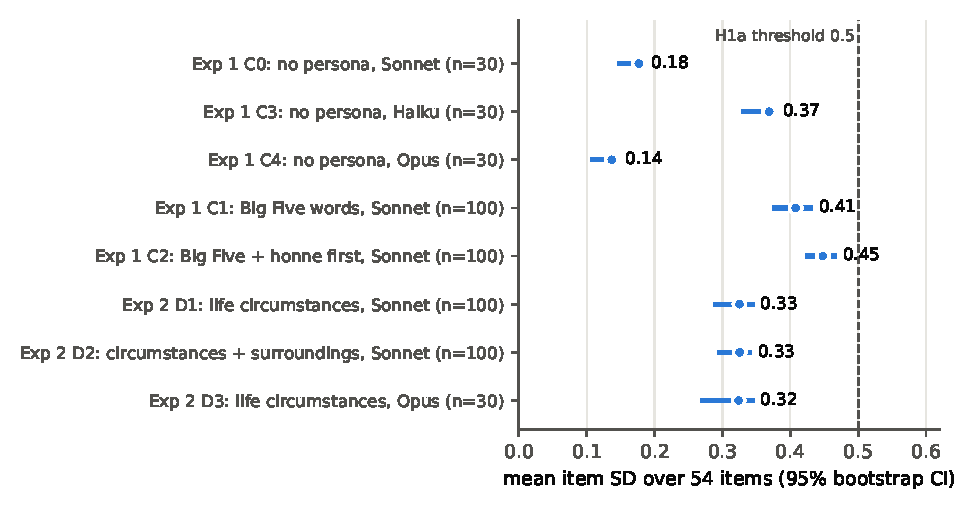
\includegraphics[width=0.75\textwidth]{figures/fig_sd.pdf}
\caption{Mean item SD across the 54 items by condition (95\% bootstrap CI). The human SDs are not available; the dashed line is the pre-registered H1a threshold.}
\label{fig:sd}
\end{figure}

\subsection{Experiment 2: life circumstances instead of personality words}

\begin{table}[!htbp]
\centering\small
\caption{Experiment 2: pre-registered hypotheses and outcomes.}
\label{tab:hyp2}
\begin{tabularx}{\textwidth}{@{}lLLl@{}}
\toprule
 & Hypothesis (threshold) & Result & Judgement \\
\midrule
H6 & PC1 share falls below Exp.~1 (D1 CI upper $<0.392$) & 0.228 [0.195, 0.312]; 0.268 inside CI & supported \\
H7 & $\ge 2$ of 5 human components reproduced (D1) & 1/5 (ownership) & \textbf{not supported} \\
H8 & Each of 4 surroundings makes gray-zone answers more lenient (coef.\ CI $<0$) & 2 of 4 (everyone; never caught) & partially supported \\
H9 & Students / strained respondents more lenient on 5 download items (diff $\le -0.2$, CI $<0$) & $-0.37$ [$-0.53$, $-0.21$] & supported \\
H10 & Strictness share falls below Exp.~1 (D1 CI upper $<0.391$) & 0.223 [0.185, 0.297] & supported \\
H11 & Opus diversifies with circumstances (D3 $-$ C4 SD, CI $>0$) & $+0.19$ [0.13, 0.22] & supported \\
\bottomrule
\end{tabularx}
\end{table}

\paragraph{A human-range first component, still a strictness dial (H6, H10, H11 supported).}
With life circumstances and no character words, Sonnet's mean item SD was 0.33 (lower than with Big Five words), but the variance was no longer dominated by one axis: first-component share 0.228 [0.195, 0.312] and strictness share 0.223 [0.185, 0.297], both with the human 0.268 inside the interval (Figure~\ref{fig:layers}a). The first component was still essentially strictness ($|r| = 0.98$), but it now carried a human-like, not an inflated, share. The largest single correlate of strictness was ``taught the rules at work or school'' ($+0.42$), followed by regular employment ($+0.35$), age ($+0.32$) and low digital literacy ($+0.31$); listening to music on free video sites ($-0.33$), being a student ($-0.28$) and having close friends ($-0.24$) went with leniency (exploratory; all 14 attributes together $R^2 = 0.65$, optimistic for $n=100$). Opus also diversified (SD 0.137 $\to$ 0.324), and the strictness of the same 30 people correlated $+0.59$ [0.34, 0.78] between Sonnet and Opus.

\paragraph{Human components still not reproduced (H7 not supported).}
D1 reproduced one human component (ownership: not returning borrowed items, joining criticism without understanding; at its sixth component), D2 one (rights awareness, at its first component), and D1+D2 none. The overall size moved into the human range, but which items move together still differs from the human sample.

\paragraph{Two of four rule-bending conditions work (H8 partially supported).}
Relative to the same person in D1, ``everyone around me does it'' shifted the gray-zone mean by $-0.21$ [$-0.26$, $-0.16$] and ``never heard of anyone caught'' by $-0.09$ [$-0.14$, $-0.03$]; ``I am in a weak position'' ($-0.01$ [$-0.07$, $+0.04$]) and ``technically easy'' ($-0.05$ [$-0.11$, $0.00$]) did not meet the criterion (Figure~\ref{fig:h8}). Adding the four lines with all conditions on the non-bending side made answers \emph{stricter} (intercept $+0.22$ [0.17, 0.27]). On the five download/copy items---the items the lines were about (exploratory)---the effects were larger ($-0.43$ and $-0.30$), and ``technically easy'' also reached $-0.16$ [$-0.27$, $-0.07$].

\paragraph{Students and strained respondents download more leniently (H9 supported).}
On the five download/copy items (A08, A09, A10, A17, A34), respondents who were students or financially strained ($n=30$) averaged 3.44 versus 3.81 for employed, non-strained respondents ($n=61$): difference $-0.37$ [$-0.53$, $-0.21$], in the direction of the thesis interviews (students cited money when downloading illegally). The difference was smaller in D2 ($-0.18$ [$-0.36$, $0.01$]) and similar for Opus D3 ($-0.31$, but with $n<15$ in one group, so not judged).

\begin{figure}[!htbp]
\centering
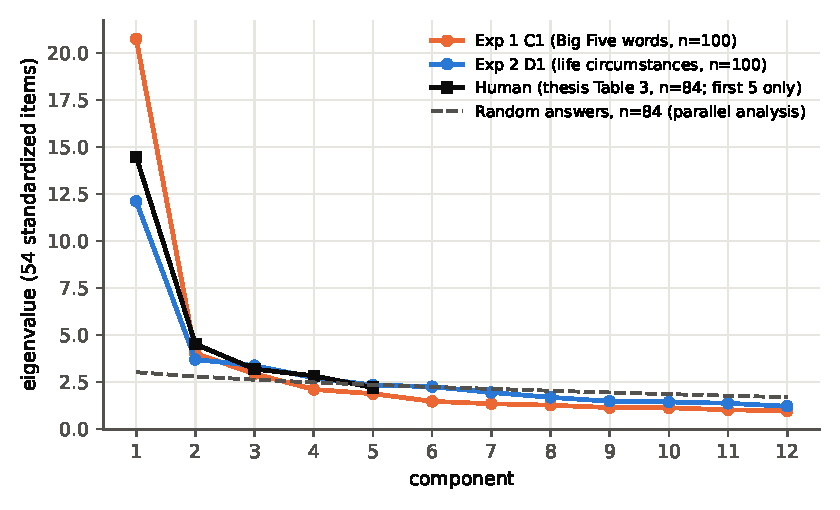
\includegraphics[width=0.62\textwidth]{figures/fig_scree.pdf}
\caption{Eigenvalues of the 54 standardized items: Big Five personas (Exp.~1 C1), life circumstances (Exp.~2 D1), the human sample (only five eigenvalues published), and random answers ($n=84$).}
\label{fig:scree}
\end{figure}

\begin{figure}[!htbp]
\centering
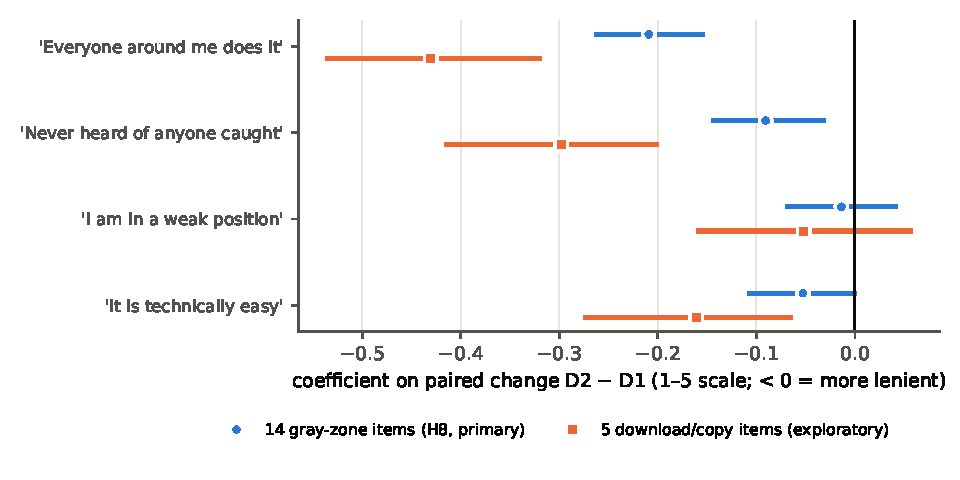
\includegraphics[width=0.75\textwidth]{figures/fig_h8.pdf}
\caption{Effects of the four ``recent surroundings'' lines (bending side vs.\ opposite side) on the within-person change from D1 to D2. Circles: pre-registered outcome (mean of 14 gray-zone items). Squares: exploratory outcome (five download/copy items). 95\% pair-bootstrap CIs.}
\label{fig:h8}
\end{figure}

\paragraph{Exploratory: what reasons did the respondents give?}
\label{sec:reasons}
This analysis was \emph{not} pre-registered as a hypothesis (the pre-registration only promised to store the reasons). We coded the 1{,}150 one-phrase reasons (5 items $\times$ 230 respondents) with a deterministic dictionary of Japanese regular expressions written after reading the reasons; no LLM was used. Codes are the thesis's seven ways of thinking (\emph{bending} side) and four rule-following reasons (illegal/rules; paying or respecting creators; relationship and courtesy; personal information). A reason can carry several codes; ``mixed'' reasons carry both a bending and a rule-following code (e.g., ``illegal, but everyone does it, so I can't say much''). 26 reasons (2\%) matched no code (mostly ``a bit bothersome'', ``borderline''). The author of the dictionary (Claude, acting for the author) read two random samples of 60 coded reasons: 57/60 (95\%) and, after fixing the errors found, 58/60 (97\%) were coded correctly; the two errors in the second sample were fixed too, so the final version has not been checked on a fresh sample. There is no second coder and no inter-rater statistic. Agreement is optimistic because the dictionary was built on the same reasons.

Reasons containing at least one rule-bending rationale made up 57\% (D1), 53\% (D2) and 31\% (D3, Opus) of reasons (same 30 people, Opus $-$ Sonnet $= -23$ points [$-35$, $-11$]); they accompanied more lenient numbers (mean answer 2.66 for bending-only, 2.96 mixed, 3.54 rule-only reasons). The most frequent bending rationales were ``where conditions are clear, act so no one is harmed'' (17--22\%; e.g., ``a friend would understand if we talk later''), ``act if the damage is tolerable'' (6--19\%), and ``follow the majority'' (5--20\%). ``An act without malice is forgivable'' appeared mainly for the unreturned clothes (18\% of B11 reasons); ``take responsibility oneself'', ``use freely if justified'' and ``interpret unclear conditions in one's favour'' were rare ($\le 4\%$). Within D2, the ``everyone does it'' line raised the share of reasons with a bending rationale from 39\% to 67\% ($+28$ points [$+18$, $+38$]) and of ``follow the majority'' by $+17$ points [$+10$, $+24$]; ``never caught'' raised them by $+11$ [$0$, $+22$] and $+9$ [$+2$, $+16$]; ``weak position'' and ``technically easy'' changed neither ($|\Delta| \le 4$ points)---the same ordering as the numeric H8 results (Figure~\ref{fig:reasons}). Overall, D2 replaced other bending rationales by ``follow the majority'' (+8 points [$+3$, $+13$]) rather than adding bending rationales ($-4$ points [$-12$, $+3$]). A caution: ``a friend would understand if we talk later'' occurred only for respondents whose description contained ``even if something happens, we can talk it over later and understand each other'' (110 of 110 cases); 83\% of A23 reasons from these respondents but 14\% from others were coded ``conditions clear''. Much of this category is the model paraphrasing its prompt---another content-matched shift.

\begin{figure}[!htbp]
\centering
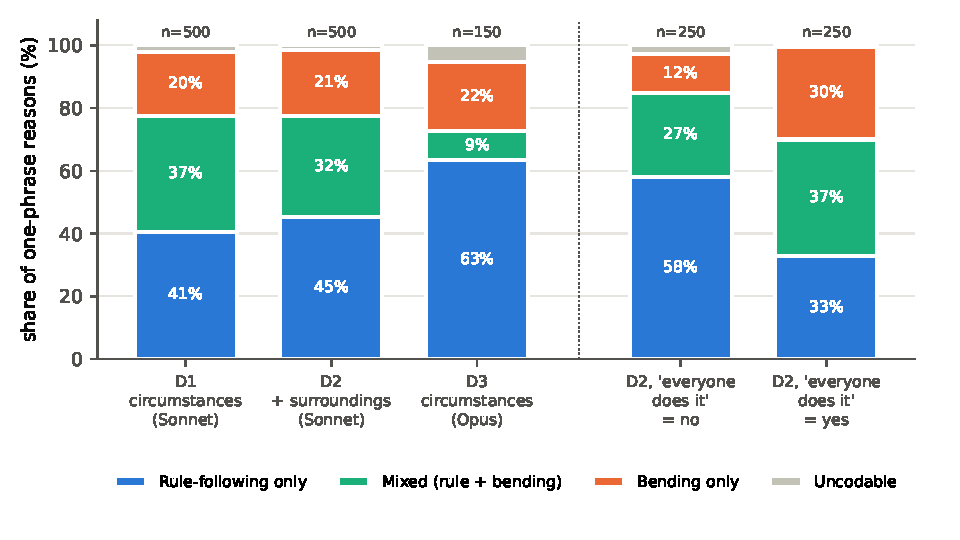
\includegraphics[width=0.75\textwidth]{figures/fig_reasons.pdf}
\caption{Exploratory dictionary coding of 1{,}150 one-phrase reasons (items A08, A09, A23, B08, B11): share of reasons with only rule-following codes, both, only rule-bending codes (the thesis's seven ways of thinking), or no code. Right: D2 split by the ``everyone around me does it'' line.}
\label{fig:reasons}
\end{figure}

\subsection{Follow-up 2b: changing the content of the surroundings, and a replication}

\begin{table}[!htbp]
\centering\small
\caption{Follow-up 2b: pre-registered hypotheses and outcomes (E1: surroundings about borrowing; D2r: repeat of D2).}
\label{tab:hyp2b}
\begin{tabularx}{\textwidth}{@{}lLLl@{}}
\toprule
 & Hypothesis (threshold) & Result & Judgement \\
\midrule
H12 & Human ownership awareness appears in E1's first two components (overlap $\ge 3$, $p<0.05$, PCs 1--2 only) & best: E1 PC2, overlap 2 (B03, B11), $p = 0.084$ & \textbf{not supported} \\
H13 & E1's first component moves away from human rights awareness (top-5 overlap $\le 1$) & E1 PC1 top 5: B09 A09 A11 A08 A16; overlap 3 & \textbf{not supported} \\
H14 & Borrowing ``everyone does it'' makes the 5 borrowing items more lenient (coef.\ $\le -0.1$, CI $<0$) & $-0.72$ [$-0.85$, $-0.58$] & supported \\
H14 & Borrowing ``never blamed'' makes the 5 borrowing items more lenient (same rule) & $-0.42$ [$-0.54$, $-0.29$] & supported \\
H15 & D2r's first component again matches rights awareness (best match PC1, overlap $\ge 3$, $p<0.05$) & PC1, overlap 3 (A08, A19, A09), $p = 0.0095$ & supported \\
\bottomrule
\end{tabularx}
\end{table}

D2's match with human rights awareness might simply have reflected that its surroundings lines were about downloading. If the first component followed the content of the surroundings, E1 should have moved it towards ownership. It did not (Table~\ref{tab:hyp2b}). The borrowing lines moved the matching answers strongly (H14 supported for both lines; ``technically easy, nobody notices'' also $-0.31$ [$-0.44$, $-0.18$], exploratory; ``weak position'', with the identical wording as in D2, $+0.08$), and the borrowing ``everyone does it'' line also loosened the download items ($-0.30$). But E1's first component still had download, Wi-Fi and office-supply items on top and overlapped human rights awareness by three (H13 not supported; without B09, whose wording is close to E1's ``taking home things from shared places'', the overlap is 2, still above the threshold). The borrowing content appeared in E1's \emph{second} component (A03 and A32 opposite to B03, B11, B06, B10), which overlapped human ownership awareness by two (H12 not supported). D2r reproduced D2's rights match (H15 supported), so it is not noise. D2 and D2r agreed on 83\% of person-item answers, and the strictness of the same person correlated $+0.79$ between them.

Exploratory: the first-component share was 0.235 [0.198, 0.291] in E1 and 0.257 [0.208, 0.327] in D2r, close to D1 (0.228) and D2 (0.250); in each, the first-component score correlated $\ge 0.98$ with the respondent's mean answer; and the first-component loading vectors of D1, D2, D2r and E1 were nearly parallel ($|\cos|$ 0.90--0.95). The top-five lists of these conditions differed only in the ordering of small loadings (about 0.18--0.23). D1 ``missed'' rights awareness (overlap 1) and D2 and D2r ``matched'' it (overlap 3) on what is essentially the same axis.

\subsection{Follow-up 2c: giving each respondent a personal history}

\begin{table}[!htbp]
\centering\small
\caption{Follow-up 2c: pre-registered hypotheses and outcomes (F1: three past events; F2: six).}
\label{tab:hyp2c}
\begin{tabularx}{\textwidth}{@{}lLLl@{}}
\toprule
 & Hypothesis (threshold) & Result & Judgement \\
\midrule
H16 & F2's PC1 share falls below D1 (paired diff.\ $\le -0.03$, CI upper $<0$) & 0.228 $\to$ 0.182; $-0.047$ [$-0.116$, $+0.006$] & \textbf{not supported} \\
H17 & F2's PC1 is no longer strictness ($|r| < 0.95$, CI upper $<0.97$) & 0.982 [0.957, 0.990] & \textbf{not supported} \\
H18 & $\ge 2$ of 5 human components reproduced in F2 & 0/5 (F1 also 0/5) & \textbf{not supported} \\
H19 & Six events lower the PC1 share more than three (F2 $-$ F1 $<0$) & $+0.012$ [$-0.034$, $+0.052$] & \textbf{not supported} \\
check & An event shifts its own domain's items (own-domain CI $>0$ in $\ge 3$ of 5 domains) & 4 of 5 (not information) & passed \\
\bottomrule
\end{tabularx}
\end{table}

The experiences were read and used locally (manipulation check passed; Table~\ref{tab:hyp2c}). An unfavourable experience made the items of its own domain stricter by $+0.16$ on average (F1 $-$ D1; mean of the five own-domain coefficients $+0.164$ [$+0.137$, $+0.193$]), while the mean effect on other domains was $+0.04$ [$+0.02$, $+0.06$], a quarter of the own-domain effect. Reasons cited the experiences: for items whose domain had an unfavourable event, 27\% of reasons carried a bending rationale, against 52\% with no event in that domain and 53\% with a favourable one (mean answers 3.35, 3.04 and 2.73). But the first component did not change in kind: its share fell from 0.228 (D1) to 0.182 (F2), a paired difference of $-0.047$ [$-0.116$, $+0.006$] (H16, not supported; the point estimate passed the threshold but the interval did not exclude 0); it still correlated 0.98 with the respondent's mean (H17, not supported); no human component was reproduced (H18, not supported); and six experiences did not spread variance more than three (H19, not supported). Its direction remained that of the earlier conditions ($|\cos|$ with D1: F1 0.91, F2 0.87). The experience domains appeared instead as clean single-domain later components: F1's third component consisted only of privacy items (A15, A23, B04, A24), and its fourth of self-responsibility (B08, B07) and information items (A29, B01). Each overlapped the corresponding human component by two, below the threshold. The human components, by contrast, mix domains (human rights awareness, for instance, contains Wi-Fi, office supplies, downloads and a copied report).

\subsection{Experiment 3: the same information inside a village}

\begin{table}[!htbp]
\centering\small
\caption{Experiment 3: pre-registered hypotheses and outcomes (numbered H1--H5, H2b in the pre-registration; prefixed ``V-'' here). L = arms with circumstances (A1+A2); control = A0 and the actual village (H0). Intervals: 95\% bootstrap.}
\label{tab:exp3}
\begin{tabularx}{\textwidth}{@{}lLlLl@{}}
\toprule
 & Hypothesis & Comparison & Result & Judgement \\
\midrule
V-H1 & Own-dispute households demand compensation more & L $-$ control & $+0.14$ [$-0.24$, $+0.50$]; 8 own-dispute answers in L & not supported \\
V-H2 & ``Around the village'' increases keeping a private store & A2 $-$ A1 & 0 (0.083 vs 0.083) & not supported \\
V-H2b & Penalty or tax proposals change & A2 $-$ A1 & 0 (none in any arm) & not supported \\
V-H3 & Wealthy--propertyless gap in keeping widens & L $-$ control & 0 (0.333 vs 0 in every arm) & not supported \\
V-H4 & Agreement within meetings falls & L $-$ control & $+0.006$ [$-0.06$, $+0.05$] & not supported \\
V-H5 & Keeping rises when the village store is low & L $-$ control & 0 & not supported \\
\bottomrule
\end{tabularx}
\end{table}

None of the six hypotheses was supported (Table~\ref{tab:exp3}). The share of representatives keeping a private store was 1 in 12 at every meeting in every arm and in the actual village (all from wealthy households: 1 in 3 of them, 0 of propertyless ones). No arm produced a penalty or tax proposal, a sharing decision, or a household leaving. The added sections were read---words about hardship and children appeared in the free-text answers of all arms---but were never copied verbatim. Exploratory observations, too few to judge: in A2, 2 of 4 own-dispute answers chose compensation (A0 1 of 9, A1 0 of 4; uninvolved households 0 in every arm), and one dispute in A2 ended unresolved, which happened in no other arm. Deaths over the three years were 22 (A0), 21 (A1), 14 (A2) and 25 (H0).

\section{Discussion}

\subsection{Two layers of variation}
\label{sec:layers}

\begin{figure}[!htbp]
\centering
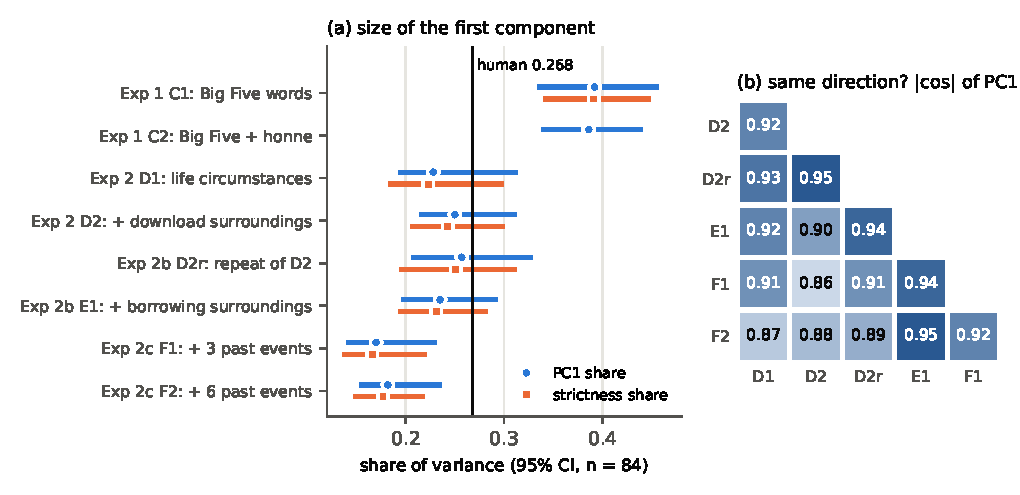
\includegraphics[width=\textwidth]{figures/fig_layers.pdf}
\caption{The strictness dial across all survey conditions with personas or life circumstances. (a) Share of standardized variance explained by the first principal component (circles) and by the single strictness composite (squares; not computed for C2), with 95\% CIs from resampling 84 respondents; vertical line: human first-component share from the thesis's first eigenvalue (14.47/54). Values are taken from the analysis of the experiment that ran each condition. (b) $|\cos|$ between first-component loading vectors of the six life-circumstance conditions (exploratory; from the 2c analysis).}
\label{fig:layers}
\end{figure}

\begin{table}[!htbp]
\centering\small
\caption{What each kind of input did: to the first component (the strictness dial) and to the matching items only. ``Same direction'': $|\cos|$ of first-component loadings with D1. Shifts are within-person changes on the 1--5 scale (negative = more lenient).}
\label{tab:layers}
\begin{tabularx}{\textwidth}{@{}lLL@{}}
\toprule
Input (condition) & First component (strictness dial) & Matching items only \\
\midrule
Big Five words (C1) & \textbf{inflated}: share 0.392 (CI excludes 0.268); $|r|$ with mean answer 0.999; strictness $+0.78$ with conscientiousness & --- \\
\emph{Honne} first (C2 vs C1) & share 0.386; whole questionnaire stricter (gray $+0.25$, others $+0.21$) & --- \\
Life circumstances (D1) & \textbf{share into human range}: 0.228 (CI contains 0.268); $|r|$ 0.983 & download items: students/strained $-0.37$ (H9) \\
+ download surroundings (D2) & not reshaped: share 0.250; same direction 0.92 & ``everyone'': gray $-0.21$, download $-0.43$; ``weak position'': gray $-0.01$ \\
Repeat of D2 (D2r) & not reshaped: share 0.257; same direction 0.93 (D2--D2r 0.95) & ``everyone'': gray $-0.18$, download $-0.35$ (exploratory) \\
+ borrowing surroundings (E1) & not reshaped: share 0.235; same direction 0.92; download items still on top & ``everyone'': borrowing $-0.72$; ``weak position'': $+0.08$; content in PC2 \\
+ 3 or 6 past events (F1, F2) & not reshaped: share 0.170, 0.182 (H16 not supported); same direction 0.91, 0.87 & own domain $+0.16$, other domains $+0.04$; single-domain later components \\
\bottomrule
\end{tabularx}
\end{table}

Taken together, the four survey experiments describe LLM respondent variation in two layers (Figure~\ref{fig:layers}, Table~\ref{tab:layers}).

\paragraph{Layer 1: a model-level strictness dial.}
In every condition in which it was computed (C1, D1, D2, D2r, E1, F1, F2), the first principal component was almost exactly the respondent's mean answer ($|r|$ 0.98--0.999), and among the six life-circumstance conditions its loading vector pointed in nearly the same direction ($|\cos|$ 0.86--0.95). What the prompt type changes is the \emph{size} of this component, not its identity. Told that a respondent is ``high in conscientiousness'', the models raise the strictness of the whole questionnaire; told ``low'', they lower it: personality words are applied as a global instruction, and the dial carries 39\% of the variance---a sharper form of the flattening described for identity prompts \citep{wang2024flatten} and of the modest persona effects reported by \citet{hu2024persona}. When the prompt instead describes a life---money, work, friends, how one listens to music---no single word drives the dial (the largest correlate is $+0.42$) and its share falls to 0.23--0.26, within the human interval. But changing the content of the surroundings (downloading vs.\ borrowing) and adding personal histories (three or six past events) left the dial in place; the share after six events (0.182) was lower, but not distinguishably so under the pre-registered rule.

\paragraph{Layer 2: local, content-matched shifts.}
On top of the dial, each piece of information moved exactly the items it was about. Download surroundings moved download items ($-0.43$ for ``everyone does it'') more than the broader gray zone ($-0.21$); borrowing surroundings moved borrowing items by $-0.72$; an unfavourable past experience made its own domain stricter by $+0.16$ with only a quarter of that reaching other domains; even the ``talk it over later'' sentence of the life descriptions re-appeared as reasons. In the component structure these shifts show up after the dial, as clean components made of the items of the domain that was put in (E1's second component; F1's privacy and self-responsibility components). The human components are not like this: each of them mixes domains, which suggests that something in a person links, say, Wi-Fi, office supplies, downloads and a copied report. Listing experiences did not create such links in our respondents.

\paragraph{Consequence (a): component ``matches'' are fragile.}
When the first component is a nearly flat strictness axis, its top five items are decided by small loading differences. C1 ``matched'' rights awareness on an axis with 53 of 54 positive loadings; D1 missed it by small loading differences; D2's match replicated in D2r but, given the shared direction, reflects download items weighing slightly more on the strictness dial rather than a separate rights awareness. Across all conditions, at most one of five human components was reproduced. Top-five overlap is a weak test of structural similarity, and conclusions from it should be read together with direction measures such as $|\cos|$ and $|r|$ with the mean answer.

\paragraph{Consequence (b): social signals shift answers, self-interest does not.}
``Everyone around me does it'' and ``I have never heard of anyone being caught'' shifted answers in both contents (H8, H14). ``I am in a weak position'' and ``it is technically easy'' had no detectable effect on gray-zone items. In the thesis, weakness (students' lack of money) and ease were reasons people gave for bending rules; the models did not convert their own disadvantage into leniency. (Ease did shift the items it most directly described in both contents---download items $-0.16$, borrowing items $-0.31$, exploratory---but weakness never did, $+0.08$ on borrowing items in E1.) This is consistent with the companion village study \citep{tanohata2026village}, where LLM agents rarely gave themselves self-serving excuses, and with LLMs' known lean toward prosocial answers \citep{mei2024turing}. In the reasons, too, D2's surroundings mainly replaced other bending rationales by ``follow the majority'' rather than adding new ones. A stable characteristic (being a student or strained, written into the life description) did make download answers more lenient (H9), so it is the \emph{momentary} self-interest line that the models ignored.

\paragraph{Consequence (c): from answers to actions, no transfer.}
Experiment~3 asked whether the information that moved survey answers also moves choices inside a society. It did not. Two explanations, not separable with these data, seem likely. First, the village offers no rule-bending choice: taking from others is a rule of the world, not a decision, so representatives choose only among rule-following actions (keep, seal, share, judge, propose, vote). Second, standing policies and precedents set at yearly meetings dominate: keeping was identical across all four runs, which suggests that the agents' memory of past policy outweighed new facts in the prompt. In the language of the two layers, the village had no item for the content-matched shift to act on. A next experiment would let villagers decide whether to take from another household's store, so that the thesis's gray zones can appear as behaviour.

\paragraph{Open question: is the human first component also strictness?}
The human first component explains 26.8\% of the variance---the same size as the LLM dial under life circumstances---and its top items (Wi-Fi, office supplies, music, video, a copied report) resemble the items that rank highest on the LLM dial. It may therefore be close to general strictness too. With only eigenvalues and top-five items published, and the raw data not available, we cannot compute its $|r|$ with the mean answer or compare loading directions. If it is strictness, the difference between LLM and human respondents lies entirely in the second layer---whether domains are linked---; if not, it already lies in the first. A new human sample on the same 54 items would settle this.

\paragraph{Asking for the id backfires.}
The thesis's model places the good-and-bad impulses (id) before censorship (superego) and adjustment (ego). Asking for a candid first impression before each answer did not expose an id; it produced a conscientious inner voice and stricter answers. Either the trained ``superego'' operates already when writing the \emph{honne}, or writing a reason commits the model to a more deliberate, norm-oriented answer. Experiment~2 therefore asked for reasons only after all numbers; we cannot tell from these data which explanation is right.

\paragraph{Back to the thesis.}
The thesis argued that humanity lies in situational adjustment between needs and norms. Our results suggest that current LLM respondents can display part of that adjustment when---and only when---the situation is written into the prompt in concrete terms, and that the adjustment follows social signals (what others do, whether anyone is caught) more readily than self-interest (weakness, ease). The two-layer picture sharpens the central open question---whether this is adjustment or the transcription of prompt cues into answers: the content-matched shifts, the ``talk it over later'' reasons and the single-domain components show that much of it is transcription onto a fixed strictness dial, and the village null result shows that, so far, it stays on paper.

\section{Limitations}
\begin{itemize}
  \item \textbf{No human raw data.} The raw data of the thesis are not available; only the published PCA table (eigenvalues and top-five items) is. We cannot compare item means, SDs, correlations or loading directions with the 84 respondents, and therefore cannot test whether the human first component is also general strictness (Section~\ref{sec:layers}). H1a and H2 use fixed thresholds or the thesis author's expectations.
  \item \textbf{Inconsistent human table.} The published cumulative proportions (0.36, \ldots, 0.81) contradict the published eigenvalues (0.268, \ldots, 0.503 if 54 standardized items). Our main reference (0.268) rests on the eigenvalues being correct.
  \item \textbf{Top-five matching is fragile.} With a nearly flat first component, small loading differences decide whether a human component ``matches'' (Section~\ref{sec:layers}); H5, H7, H12, H13, H15 and H18 inherit this weakness. $|\cos|$ between loading vectors was added after the 2b data were seen and is exploratory.
  \item \textbf{One model for the follow-ups; one run each.} Follow-ups 2b and 2c used Sonnet only. Each condition was run once, except D2, which was repeated as D2r; D2 and D2r agreed on 83\% of person-item answers, so single runs carry noticeable sampling variation. H16's point estimate passed its threshold while its interval did not; a larger sample might change that judgement.
  \item \textbf{Prompts written by Claude; assumed distributions.} The life descriptions, the surroundings lines, the 20 past events and one sentence of the instructions were written by Claude for the author; the event domains were chosen to match the thesis's five awareness names (so an event domain moving its items is partly by construction). Attributes and events were assigned by assumed distributions (often half and half), not by real frequencies; some attributes (``taught the rules'', ``a creator in the family'') are close cues to the answers. The 2016 sample consisted of acquaintances of the author and their referrals; it is neither random nor representative, and our simulated respondents do not mirror it.
  \item \textbf{Possible contamination.} Models may have seen many information-ethics questionnaires and their ``correct'' answers. The thesis itself is, to our knowledge, not public.
  \item \textbf{Platform.} Respondents were Claude Code workflow agents, not raw API calls; agent instructions may affect answers; temperature could not be set; model versions behind aliases were not recorded.
  \item \textbf{Japanese only, single item order, one survey.} The 2016 items mention CDs, rental videos and chain mail, which are dated. Experiment~2 also added the post-hoc reasons request, so differences from Experiment~1 are not solely due to persona format.
  \item \textbf{Reasons coding} is exploratory, single-coder, dictionary-based and built on the same data it was evaluated on.
  \item \textbf{Village experiment.} One copy per arm and three simulated years (three yearly meetings at which policy can change); few own-dispute answers; no rule-bending action available to agents; the first-step collection failure in A2. The actual village (H0) was run before code added later (a switch for distant traders), but the same days replay byte-identically with the new code.
\end{itemize}

\section{Ethics}
The 2016 survey promised respondents that data would be statistically processed and no individual identified; the interviews promised anonymous use for the thesis only and disposal afterwards. In line with these promises, this paper uses only the thesis's published aggregate results (the PCA table and the published list of ways of thinking and conditions). No raw survey answers and no interview material were used. No new human participants were recruited. \emph{LLM use:} the simulated respondents were Claude models; the analysis code, figures, reasons dictionary, the prompts given to the simulated respondents, and the first draft of this manuscript were produced with the assistance of Claude (Anthropic) via Claude Code, under the author's direction; the author is responsible for the content. \todo{author: confirm the 2016 consent wording and that publishing aggregates is acceptable to your former institution.}

\section{Data and code availability}
Everything is in the public repository \url{https://github.com/Ryo-Tanohata/RobotSimulaterRyo}. \emph{Pre-registrations} (\texttt{docs/research/humanity/paper2\_exp*\_prereg.md}), each committed before any model was run: Experiment~1 \texttt{2c8f966c}; Experiment~2 \texttt{b88ad84c}; Follow-up 2b \texttt{2b8ffb0b} (final check fixed at \texttt{abbd853b}); Follow-up 2c \texttt{154ae7f0} (final check fixed at \texttt{ea33980d}); Experiment~3 \texttt{b1c1ae8a}. \emph{Results} (\texttt{paper2\_exp*\_results.md}) at commits \texttt{3ba2764d} (Exp.~1), \texttt{e58e9560} (Exp.~2), \texttt{d2a84953} (2b), \texttt{0eab21f6} (2c) and \texttt{f471bb58} (Exp.~3). \emph{Surveys} (\texttt{sim/society/tools/survey/}): questionnaires, personas, life descriptions, surroundings lines and past events; workflow scripts; all 920 raw answers (\texttt{answers/}, \texttt{answers\_exp2/}, \texttt{answers\_exp2b/}, \texttt{answers\_exp2c/}) with 3{,}150 one-phrase reasons (Experiment~2: 1{,}150; 2b and 2c: 1{,}000 each); analysis scripts \texttt{analyze.py}, \texttt{analyze\_exp2.py}, \texttt{analyze\_exp2b.py}, \texttt{analyze\_exp2c.py} and \texttt{reasons\_codebook.py}; outputs in \texttt{out/}, \texttt{out\_exp2/}, \texttt{out\_exp2b/}, \texttt{out\_exp2c/}. \emph{Village}: code \texttt{sim/society/exp3.py} and \texttt{sim/society/tools/exp3\_*} (measures: \texttt{exp3\_measure.py}), village copies \texttt{sim/society/data\_E3\_A0\_1}, \texttt{\_A1\_1}, \texttt{\_A2\_1}, measures in \texttt{docs/research/humanity/data/exp3/}. Figures and the item table are regenerated by \texttt{paper/paper2/figures/make\_figures.py} and \texttt{make\_tables.py}. \todo{author: archive a tagged release (e.g., Zenodo DOI).}

\bibliographystyle{plainnat}
\bibliography{refs}

\clearpage
\appendix
\section{Items}
{\small
\begin{longtable}{@{}l>{\raggedright\arraybackslash}p{0.50\textwidth}rrrrr@{}}
\caption{The 54 items (English gloss; the questionnaire was administered in Japanese), the thesis's expected ``common-sense'' answer (norm; 5 = serious problem, 1 = no problem at all), and LLM item means. $\dagger$ = gray-zone item (14). C0/C4: Experiment 1 without persona (Sonnet/Opus, $n=30$); C1: Big Five words (Sonnet, $n=100$); D1: life circumstances (Sonnet, $n=100$).}\label{tab:items}\\
\toprule
Item & Behaviour & Norm & C0 & C4 & C1 & D1 \\
\midrule
\endfirsthead
\toprule
Item & Behaviour & Norm & C0 & C4 & C1 & D1 \\
\midrule
\endhead
A01$^\dagger$ & Watching a film still in cinemas after finding it posted online & 2 & 2.10 & 4.20 & 2.20 & 2.32 \\
A02 & Making the data of a DVD one bought viewable by anyone online & 4 & 4.97 & 5.00 & 4.65 & 4.86 \\
A03 & Posting images of a favourite celebrity on one's blog without permission & 1.5 & 3.00 & 4.00 & 3.03 & 3.09 \\
A04$^\dagger$ & Copying a detailed web page verbatim and submitting it as a report & 3 & 5.00 & 5.00 & 4.49 & 4.80 \\
A05 & Using someone else's smartphone to buy paid lottery items in a game app & 5 & 5.00 & 5.00 & 4.99 & 4.99 \\
A06 & Looking through someone's phone address book without permission to learn about their acquaintances & 5 & 4.00 & 5.00 & 4.12 & 4.19 \\
A07$^\dagger$ & Scanning part of a book one owns and making it viewable by anyone online & 2 & 4.27 & 5.00 & 4.28 & 4.38 \\
A08$^\dagger$ & Downloading music from a commercial CD for free from an individual's website & 5 & 4.07 & 4.90 & 3.81 & 3.67 \\
A09$^\dagger$ & Downloading a live video of a favourite singer that someone uploaded to YouTube & 3 & 3.03 & 3.93 & 3.05 & 3.06 \\
A10 & Copying commercial software onto DVD or CD & 5 & 4.67 & 4.00 & 4.21 & 4.41 \\
A11 & Photographing only the needed pages of a book in a bookshop instead of buying it & 4 & 3.93 & 4.00 & 3.59 & 3.81 \\
A12 & Photographing the contents of a library book & 1 & 2.13 & 2.47 & 2.19 & 2.16 \\
A13 & Selling counterfeit brand bags or watches in an online auction & 5 & 5.00 & 5.00 & 5.00 & 5.00 \\
A14 & Using someone else's mobile phone for a call without particularly asking & 5 & 2.80 & 3.27 & 2.52 & 2.44 \\
A15 & Giving someone's phone number or e-mail address to others without permission & 5 & 4.00 & 4.90 & 3.65 & 3.83 \\
A16 & Asking for and using a colleague's PC password at work & 5 & 4.00 & 4.00 & 3.74 & 3.93 \\
A17 & Sending the data of a purchased music CD to a friend (cloud or CD-R) & 4 & 3.87 & 4.00 & 3.44 & 3.59 \\
A18$^\dagger$ & Making derivative works without permission (character paint on one's car, cosplay) & 2 & 2.93 & 3.00 & 2.74 & 2.99 \\
A19 & Using a Wi-Fi password one learned by chance to connect one's PC & 4 & 4.00 & 4.00 & 3.70 & 3.95 \\
A20$^\dagger$ & Posting a photo showing strangers' faces to one's SNS or web page as is & 2 & 3.00 & 3.97 & 2.88 & 2.96 \\
A21 & Using CC instead of BCC when e-mailing many people & 5 & 3.00 & 4.00 & 2.89 & 2.98 \\
A22 & Scanning an interesting magazine page and e-mailing it to a friend & 1 & 3.00 & 3.57 & 2.86 & 3.02 \\
A23$^\dagger$ & Posting a photo taken with a friend on one's SNS without the friend's permission & 2 & 3.07 & 3.97 & 2.91 & 2.71 \\
A24 & Complaining about work on one's web page, naming another person & 5 & 4.00 & 4.90 & 4.06 & 4.02 \\
A25 & Using a PC on which someone else is still logged in to Google or Yahoo! & 4 & 3.90 & 4.00 & 3.50 & 3.63 \\
A26 & Following a chain mail's request to forward it to many people & 4 & 2.13 & 3.60 & 2.06 & 2.22 \\
A27$^\dagger$ & Happening to see someone typing their PC password & 2 & 1.90 & 2.00 & 1.82 & 1.93 \\
A28 & Making one's own copy of goods seen on TV or in town, after looking them up & 1 & 1.13 & 2.00 & 1.32 & 1.54 \\
A29$^\dagger$ & Posting an opinion from someone else's blog verbatim on one's own blog & 2 & 4.00 & 4.00 & 3.91 & 3.97 \\
A30 & Registering for an app a friend recommended on SNS without checking it & 1 & 3.00 & 3.00 & 2.84 & 2.95 \\
A31 & Giving one's own auction item a better rating than it deserves & 5 & 5.00 & 5.00 & 4.42 & 4.54 \\
A32 & Picking arguments in a group chat to drive out someone who disagrees & 5 & 4.00 & 4.00 & 4.04 & 3.99 \\
A33 & Joining others in a group chat in criticising someone without understanding the issue & 5 & 4.00 & 4.63 & 4.13 & 4.01 \\
A34 & Dubbing a DVD rented from a video shop at home & 4 & 3.80 & 3.63 & 3.51 & 3.71 \\
A35 & Criticising a restaurant as bad on one's blog & 1 & 2.67 & 3.00 & 2.76 & 2.99 \\
B01 & Copying another person's report verbatim when given the chance & 5 & 5.00 & 5.00 & 4.67 & 4.88 \\
B02 & Copying answers seen on another person's sheet during a test & 4 & 5.00 & 5.00 & 4.70 & 4.96 \\
B03 & Keeping something borrowed and not returning it & 5 & 4.00 & 4.00 & 3.97 & 4.01 \\
B04 & Telling a mutual friend a friend's personal details (birthday, address) when asked & 1 & 3.63 & 3.97 & 3.52 & 3.47 \\
B05 & Drawing or pasting Disney characters on one's pencil board or notebook & 1 & 1.97 & 2.00 & 1.92 & 1.98 \\
B06 & Joining others at school or work in criticising someone without understanding the issue & 4 & 4.00 & 4.63 & 4.12 & 4.01 \\
B07 & Throwing away New Year cards and letters as they are & 1 & 2.73 & 3.00 & 2.60 & 2.76 \\
B08$^\dagger$ & Throwing away a mail-order box with the shipping label still attached & 1 & 2.97 & 3.00 & 2.74 & 2.97 \\
B09 & Taking office supplies home because one needs them & 5 & 4.13 & 5.00 & 4.01 & 4.09 \\
B10 & Keeping a CD borrowed from a friend because they have not asked for it & 5 & 3.00 & 3.87 & 3.10 & 3.01 \\
B11$^\dagger$ & Not having returned clothes borrowed when staying over at a friend's & 5 & 3.17 & 4.00 & 3.21 & 3.03 \\
B12 & Passing off an opinion heard from someone else as one's own & 4 & 3.40 & 3.00 & 3.36 & 3.06 \\
B13$^\dagger$ & Picking and eating fruit from a tree in a neighbour's garden & 3 & 4.00 & 4.47 & 3.83 & 3.97 \\
B14 & Writing a memo on a public-toilet wall during an urgent call (only a pen at hand) & 5 & 3.00 & 4.07 & 3.12 & 3.11 \\
B15$^\dagger$ & Walking past when the person ahead drops what look like documents & 2 & 3.00 & 3.07 & 2.93 & 2.94 \\
B16 & Taking an empty seat on a crowded bus or train without hesitation & 4 & 1.13 & 1.97 & 1.40 & 1.38 \\
B17 & Sometimes playing loud music late at night & 5 & 4.00 & 4.10 & 3.85 & 3.93 \\
B18 & Often forgetting to return library books & 5 & 3.00 & 4.00 & 3.00 & 2.94 \\
B19 & Forgetting to return a DVD rented from a video shop & 4 & 2.50 & 4.00 & 2.83 & 2.63 \\
\bottomrule
\end{longtable}

}

\end{document}
